\chapter{Pipeline and Results}
This chapter introduces the pipeline of the \textit{in silico} data set (Figure 3.3, Figure 3.8) and the pipeline for the Dream8 Challenge data set describing the processing of the data from discretization to inferring a network and finally scoring the predicted network against a gold standard network. The results of the \textit{in silico} data set are necessary to set the paramter for the Dream8 Challenge pipeline. Both pipelines can be executed from the command line by a bash script and are available on Git: "github.com/ninakersten/Masterthesis". 

\section{Pipeline of the \textit{in silico} data set}

For both the subnetworks and the cell cycle network continous data sets ($S=\{ S_{1},S_{2},...,S_{n}\} $) are generated with \textit{odefy}, a MATLAB- and Octave-compatible toolbox for the automated tansformation of Boolean models into systems of ordinary differential equations \citep{Krumsiek2010}. With \textit{odefy} the number of sample points and the time interval for a data simulation can be determined. The time interval is set to a range of 1 to 50. For later application of the Dream8 Challenge data set the \textit{in silico} data sets are converted into the CSV format in the structure of the Dream8 Challenge input data (Table 2.8) and for the discretization and learning step converted into a text file format (Figure 3.1). The species' names are anonymized by single character depicted in the first header of a \textit{txt} file and original names are stored in a header below followed by the time course data set \textit{S}.

%\noindent See the following command :
%\begin{lstlisting}[language=bash]
%  $ bash insilico.sh 100 KM3 BESTFIT
%\end{lstlisting}

%bild zeigen, wie die Daten in dem file angeordnet sind.
\begin{figure}[H]
\captionsetup{width=1.0\linewidth}
\centering
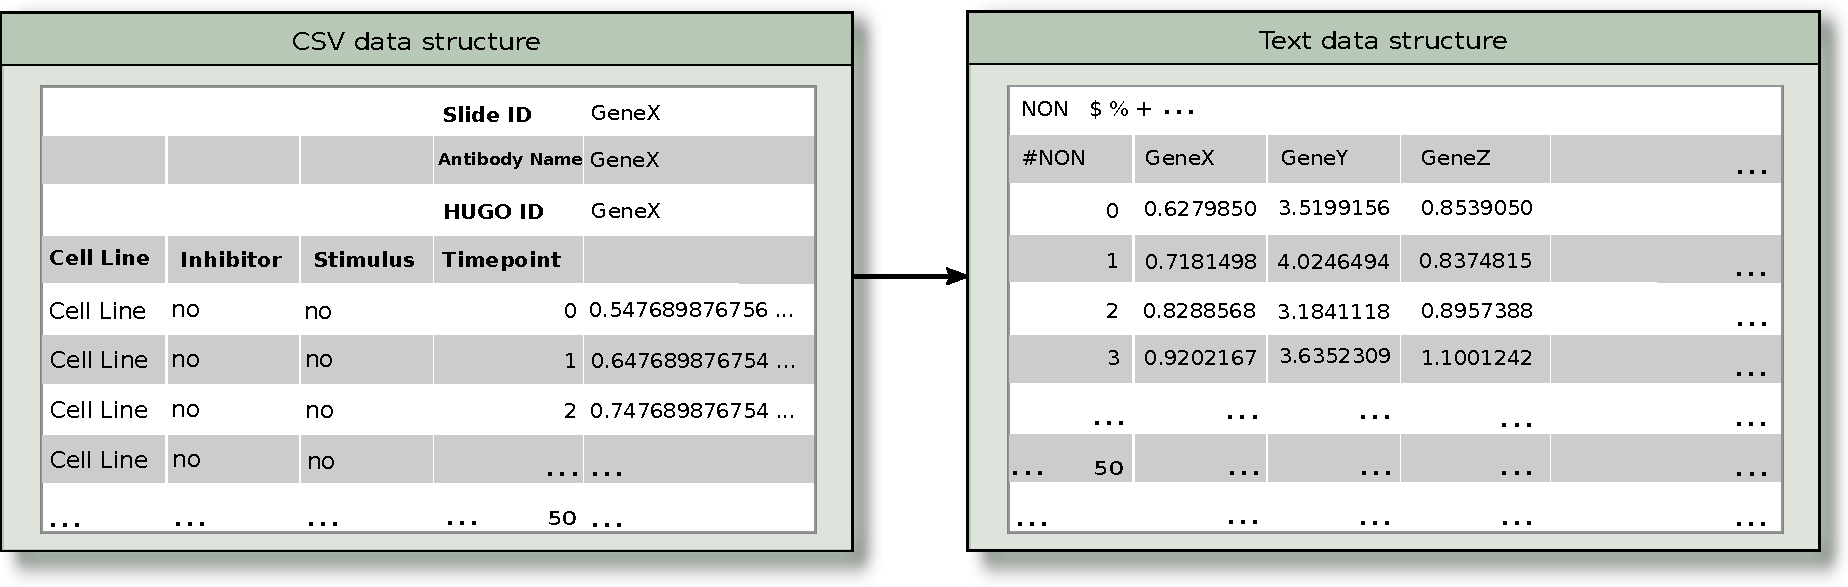
\includegraphics[width=1.0\textwidth]{./Bilder/CSV2TXT.pdf}
\caption[CSV to TXT]{\textbf{CSV to TXT:} Anonymized single character represent the species and information about cell line,inhibitor and stimulus is neglected. }
\label{fig:9}
\end{figure}


After discretizing continous time course data into a set of binary values ($B=bin(S)$, where $bin\in \{ $2-k-means, iterative k-means$\}$) redundant values are removed from this set. Boolean networks ($N=learn(B)$) are learned from this data by each inference algorithm ($learn\in \{$Best-Fit, Full-Fit, Reveal$\}$). A value for the minimal error $MinError$ is set, sucht that the inference algorithms runs i times until a network with an error ($Error(N,B)$) lower that the minimal error is achieved. It is worthwhile to get an error of $0$, meaning the the boolean model describes the data perfectly. The amount of returned solutions is set to a value of $3$, such that in each inference process three solutions (resp. Boolean Networks) are inferred, all with an error lower than the minimal error. A single Boolean Network with the lowest error across all iterations is selected for further processing.\\
For investigating the impact of the \textit{in-degree} in a network on the algorithms performance, the E.Coli subnetworks are processed by the iterative k-means clustering algorithm with a cluster depth of $d=3$ in combination with Best-fit, Full-fit or Reveal. The cluster depth with $d=3$ is selected due to previous research proving its reliablity regarding the trade off between simplicity and loss of information (e.g. oscillations).\\
%Quelle: TS2B Paper
For assessing the dependence of an inference algorithm to the number of sample points, the continous data for the cell cycle is generated for $m\in\{ 50$, $100$, $150$, $200$, $250$, $300$, $350$, $400$ ,$450$, $500\}$. Starting by a number of 50 sample points is due to the fact, that with lower amount the inference algorithms can not run. And for measuring the impact of the clustering depth the cell cycle's continous data is generated with 100 sample points (similar to the abundance of sample points of $\sim 85$ in the Dream8 Challenge) and inferred with a clustering depth of $d=\{ 1,2,3,4,5,6,7,8,9,10\}$. In Table 3.1 shows a summerized overview of these settings.

\begin{table}[H]
%\resizebox{\textwidth}{!}{
%{\tabcolsep=6pt%
\begin{center}
%\captionsetup{width=0.87\linewidth}
%\small
\begin{tabular}{l|l|l}
\toprule 
 & E.coli & Cell cycle \\
 \hline\hline
\# networks & $45$ & $1$\\
\rowcolor{black!10} \# nodes & $\{10,11,12,13,14\}$ & $10$\\
max. \textit{indegree} & $\{1,2,3,4,5,6,7,8,9\}$ & $5$\\
\rowcolor{black!10} \# sample points & $100$ & $\{50,100,150,200,250,300,350,400,450,500\}$\\
cluster depth & $3$ & $\{1,2,3,4,5,6,7,8,9,10\}$\\
\rowcolor{black!10} Best-fit & \checkmark & \checkmark \\
 					Full-Fit & \checkmark & \checkmark \\
\rowcolor{black!10} Reveal & \checkmark & \checkmark \\
\bottomrule
\end{tabular}
\captionof{table}{\textit{In silico:} Setting Table}
\end{center}
%}
\end{table}  

The predicted networks are converted (from bnet format) to interaction graphs (to a sif format) by PyBoolNet (Figure 4.2). Each predicted interaction graph is scored against a gold standard interaction graph generated from the initial boolean network with PyBoolNet. Hence each line in a SIF-format of an interaction graph represents an edge of the graph (Figure 4.2). The edges of the gold standard and the prediction are compared resulting in a confusion matrix for computing Precision, Recall, Accuracy, Balanced Accuracy and the Matthew Correlation Coeffiecient.

\begin{figure}[H]
\centering
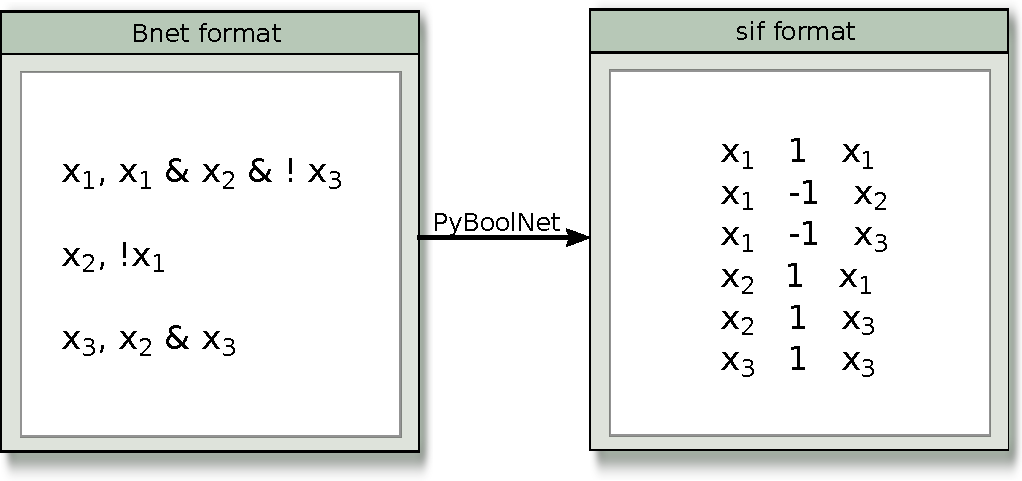
\includegraphics[width=0.7\textwidth]{./Bilder/bnet2sif.pdf}
\caption[Boolean Network to Interaction Graph]{\textbf{Boolean Network to Interaction Graph:} The predicted Boolean Network $N$ is converted into the Interaction Graph $IG$.}
\label{fig:9}
\end{figure}

 

\begin{figure}[H]
\centering
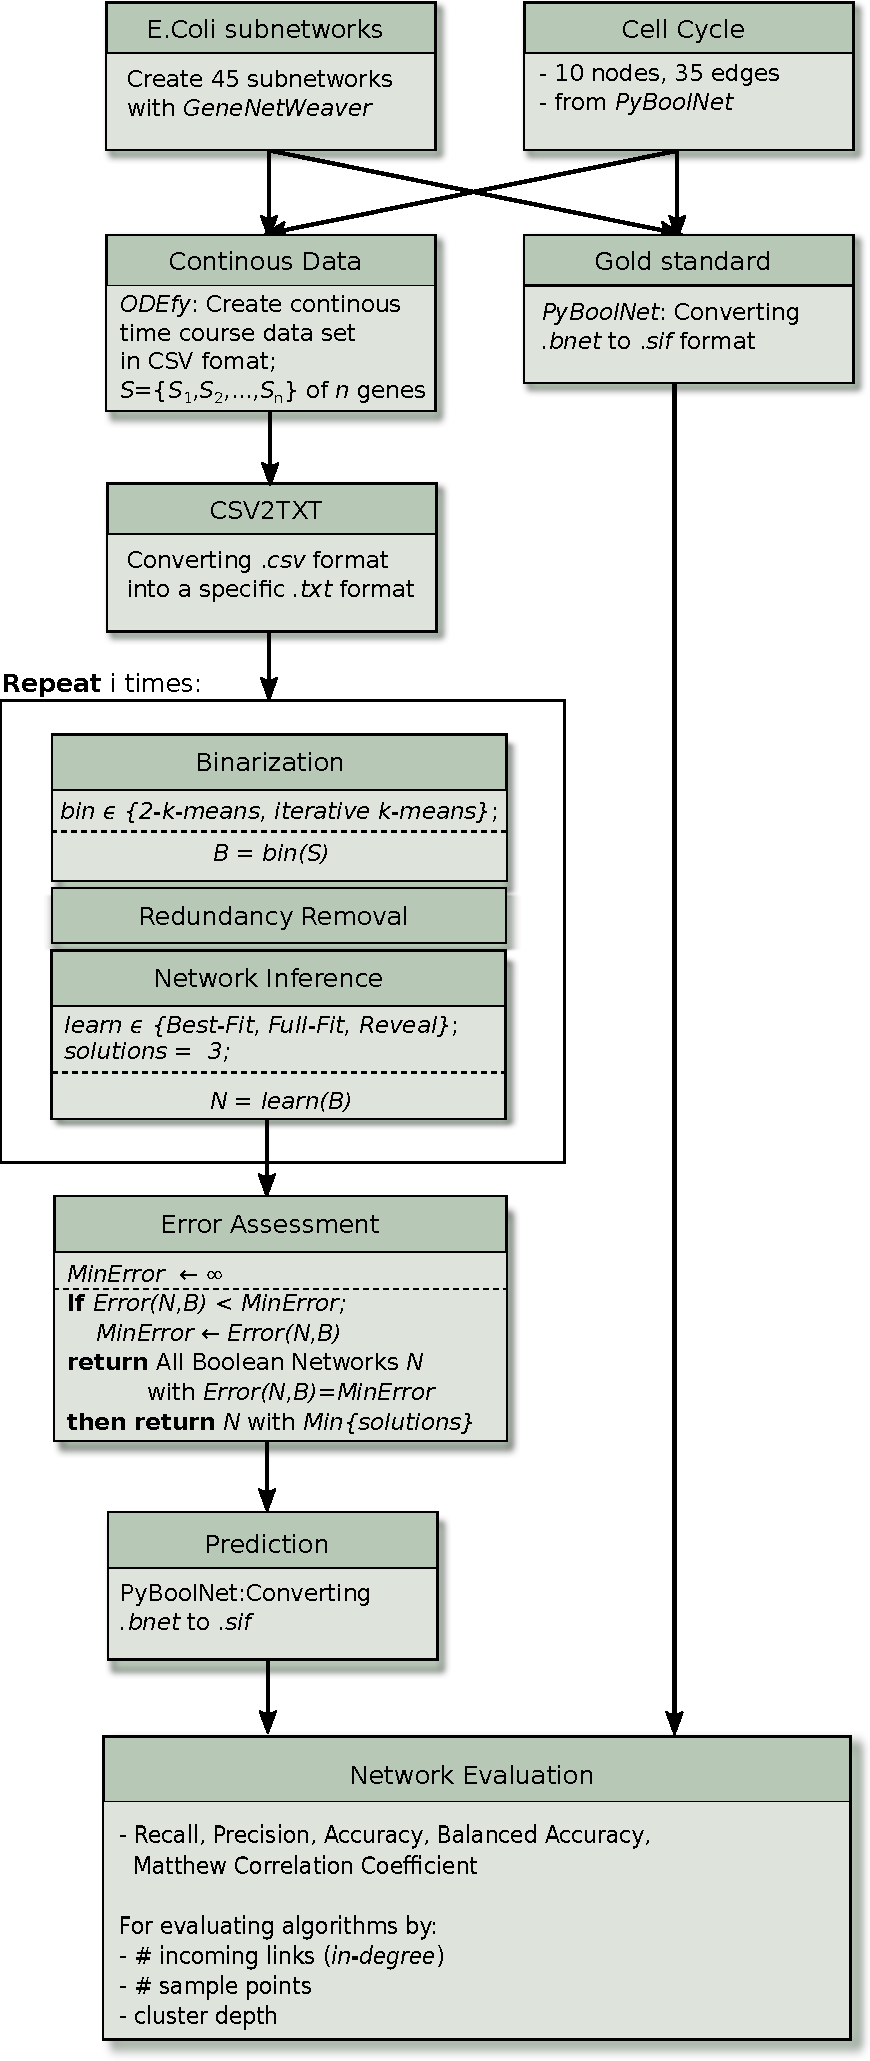
\includegraphics[width=0.55\textwidth]{./Bilder/pipeline_insilico.pdf}
\caption[\textit{In silico} Pipeline]{\textbf{Pipeline \textit{in silico}.}}
\label{fig:9}
\end{figure}



\section{Results of the \textit{in silico} data set}
\subsection*{In-degree}
The subnetworks of E.Coli are grouped into nine categories, each containing five subnetworks with 10,11, 12, 13 and 14 nodes. A category denote the number of incoming links (resp. in-degree) of each node in a network. The Figure 4.4 shows the scoring result of the 45 subnetworks by the average structure accuracy. Increasing the in-degree causes an decreasing of the accuracy. 

\begin{figure}[H]
\centering
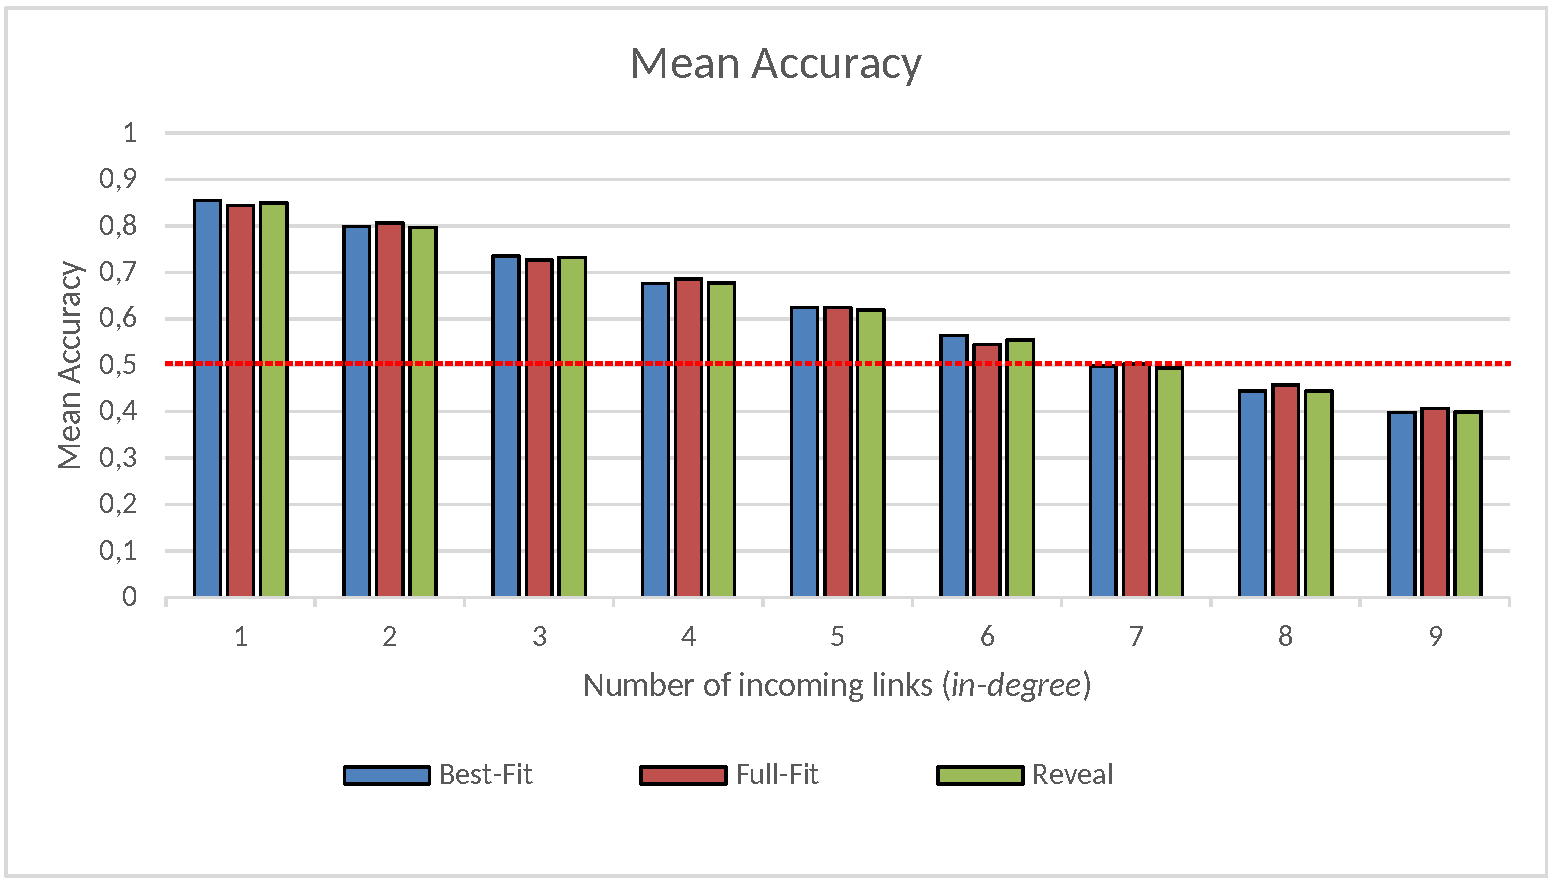
\includegraphics[width=0.9\textwidth]{./Bilder/Scoring/insilico/1_Indegree_Runtime/MeanAcc_indegree.pdf}
\caption[Average Structure Accuracy]{\textbf{Average Structure Accuracy.} E.Coli subnetworks are grouped into nine groups definded by the in-degree of the nodes in a subnetwork. With increasing in-degree the average accuracy of all three inference algorithms decreases. }
\label{fig:}
\end{figure}



Thus the more nodes occure with a high in-degree the more complex is the system and the worse the inference algorithm is able to detect the whole information. This observation covers the observation of \citep{10.1371/journal.pone.0171097}, where the settings where slightly different. instead of grouping sets of networks, they grouped the nodes of about 300 networks with different network sizes ($|V| = 10,20,$...$100$).\\

\subsection*{Number of sample points}
For the cell cycle continous data different sets with different number of sample points $\{50,100,150,200,250,300,350,400,450,500\}$ are generated. The resulting networks are tested by accuracy, precision, recall and Mathew correlation coefficient. The Figure 4.5 shows that changing the amount of sample point does not change significantly the performance of the algorithms.

\begin{figure}[H]
\centering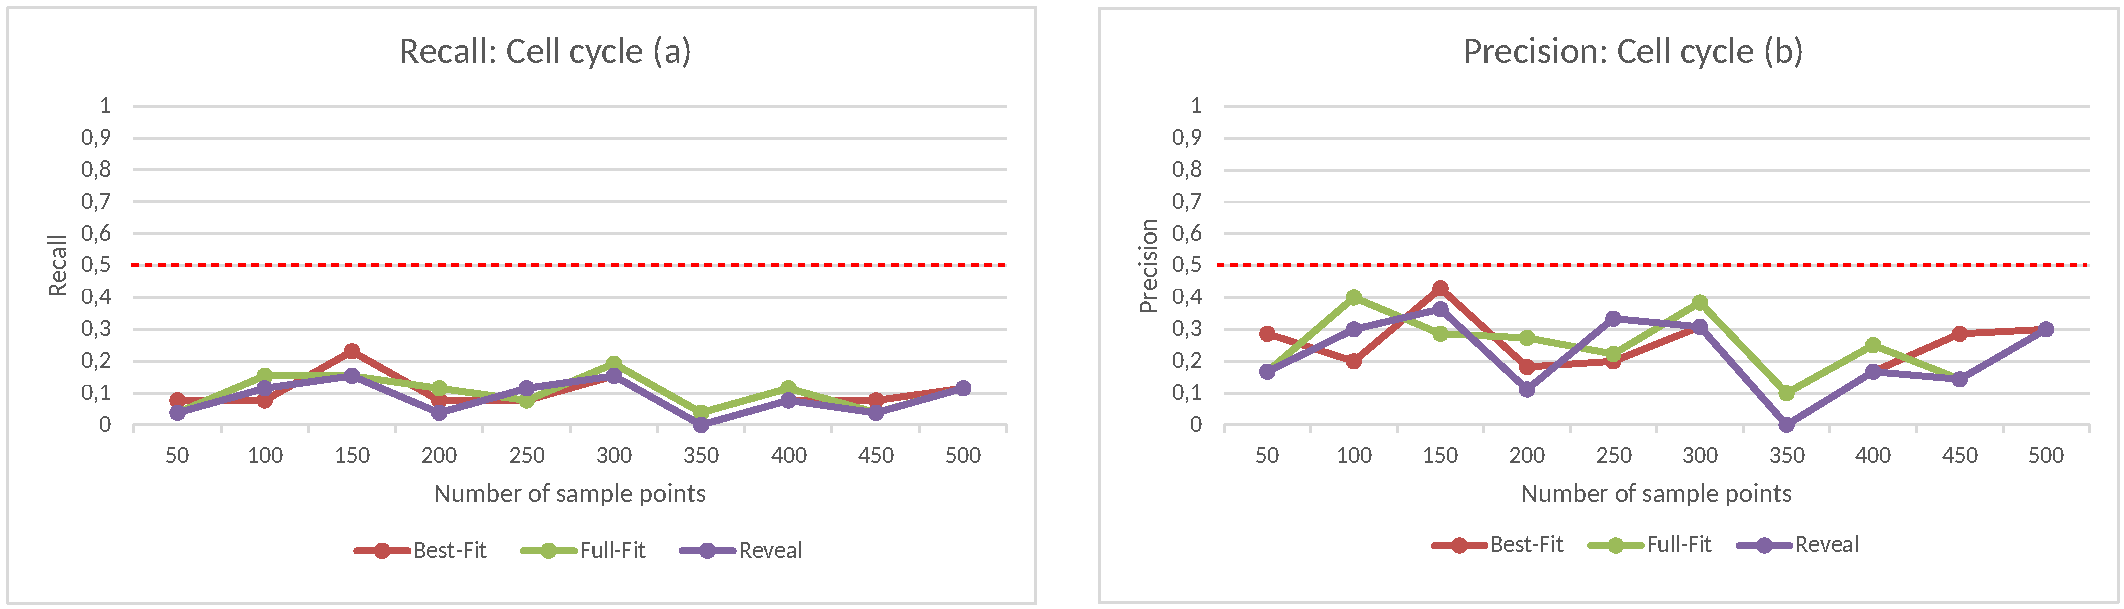
\includegraphics[width=0.9\textwidth]{./Bilder/Scoring/insilico/2_cellcycle_measurements/RecPrec.pdf}
\caption[NumberOfPoints]{\textbf{Number of sample points.}In (a) the accuracy ranges around a value of $0.7$, whereas Precision (c) and Recall (d) range on a low level of $0,3$ to $0,4$. Despite a few insignificant fluctuations the value almost alway stays the same. In (b) the mcc does not change either.}
\label{fig:}
\end{figure}

\begin{figure}[H]
\centering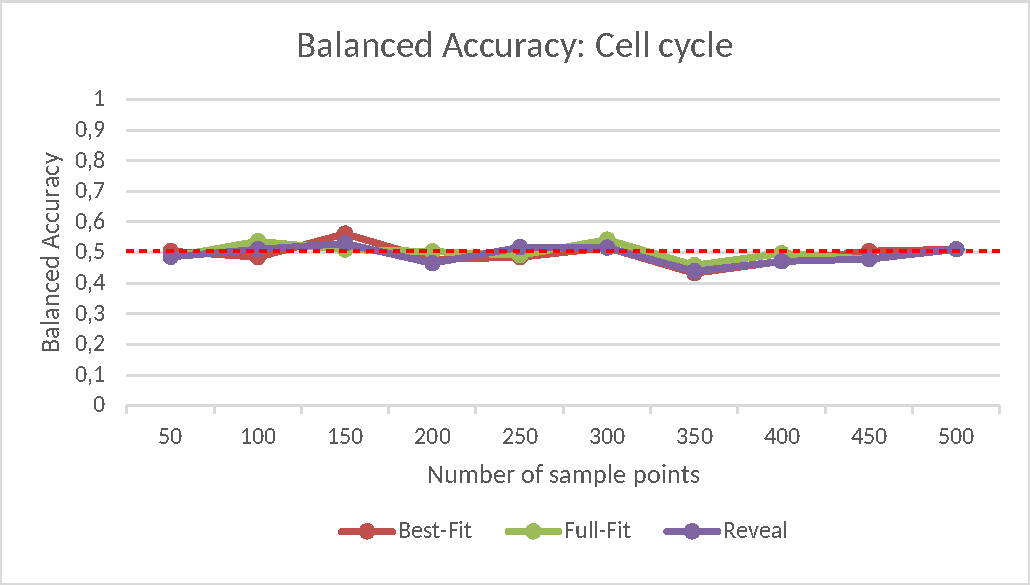
\includegraphics[width=0.9\textwidth]{./Bilder/Scoring/insilico/2_cellcycle_measurements/Bacc.pdf}
\caption[NumberOfPoints]{\textbf{Number of sample points.}In (a) the accuracy ranges around a value of $0.7$, whereas Precision (c) and Recall (d) range on a low level of $0,3$ to $0,4$. Despite a few insignificant fluctuations the value almost alway stays the same. In (b) the mcc does not change either.}
\label{fig:}
\end{figure}

\subsection*{Cluster depth}
Changing the cluster depth of the iterative k-means clustering algorithm changes the performance of the algorithms not significantly. As mentioned in (Paper),the iterative k-means clustering algorithms captures the oszillations (resp. kind of dynamic) in a system in contrast to the two cluster k-means algorithm. Beside the fact only the structure of a network not the dynamics are analyzed later network inference is performed with the iterative k-mean clustering method with a recommanded clustering depth of $d=3$ (Paper).
%Paper of TS2B
\begin{figure}[H]
\centering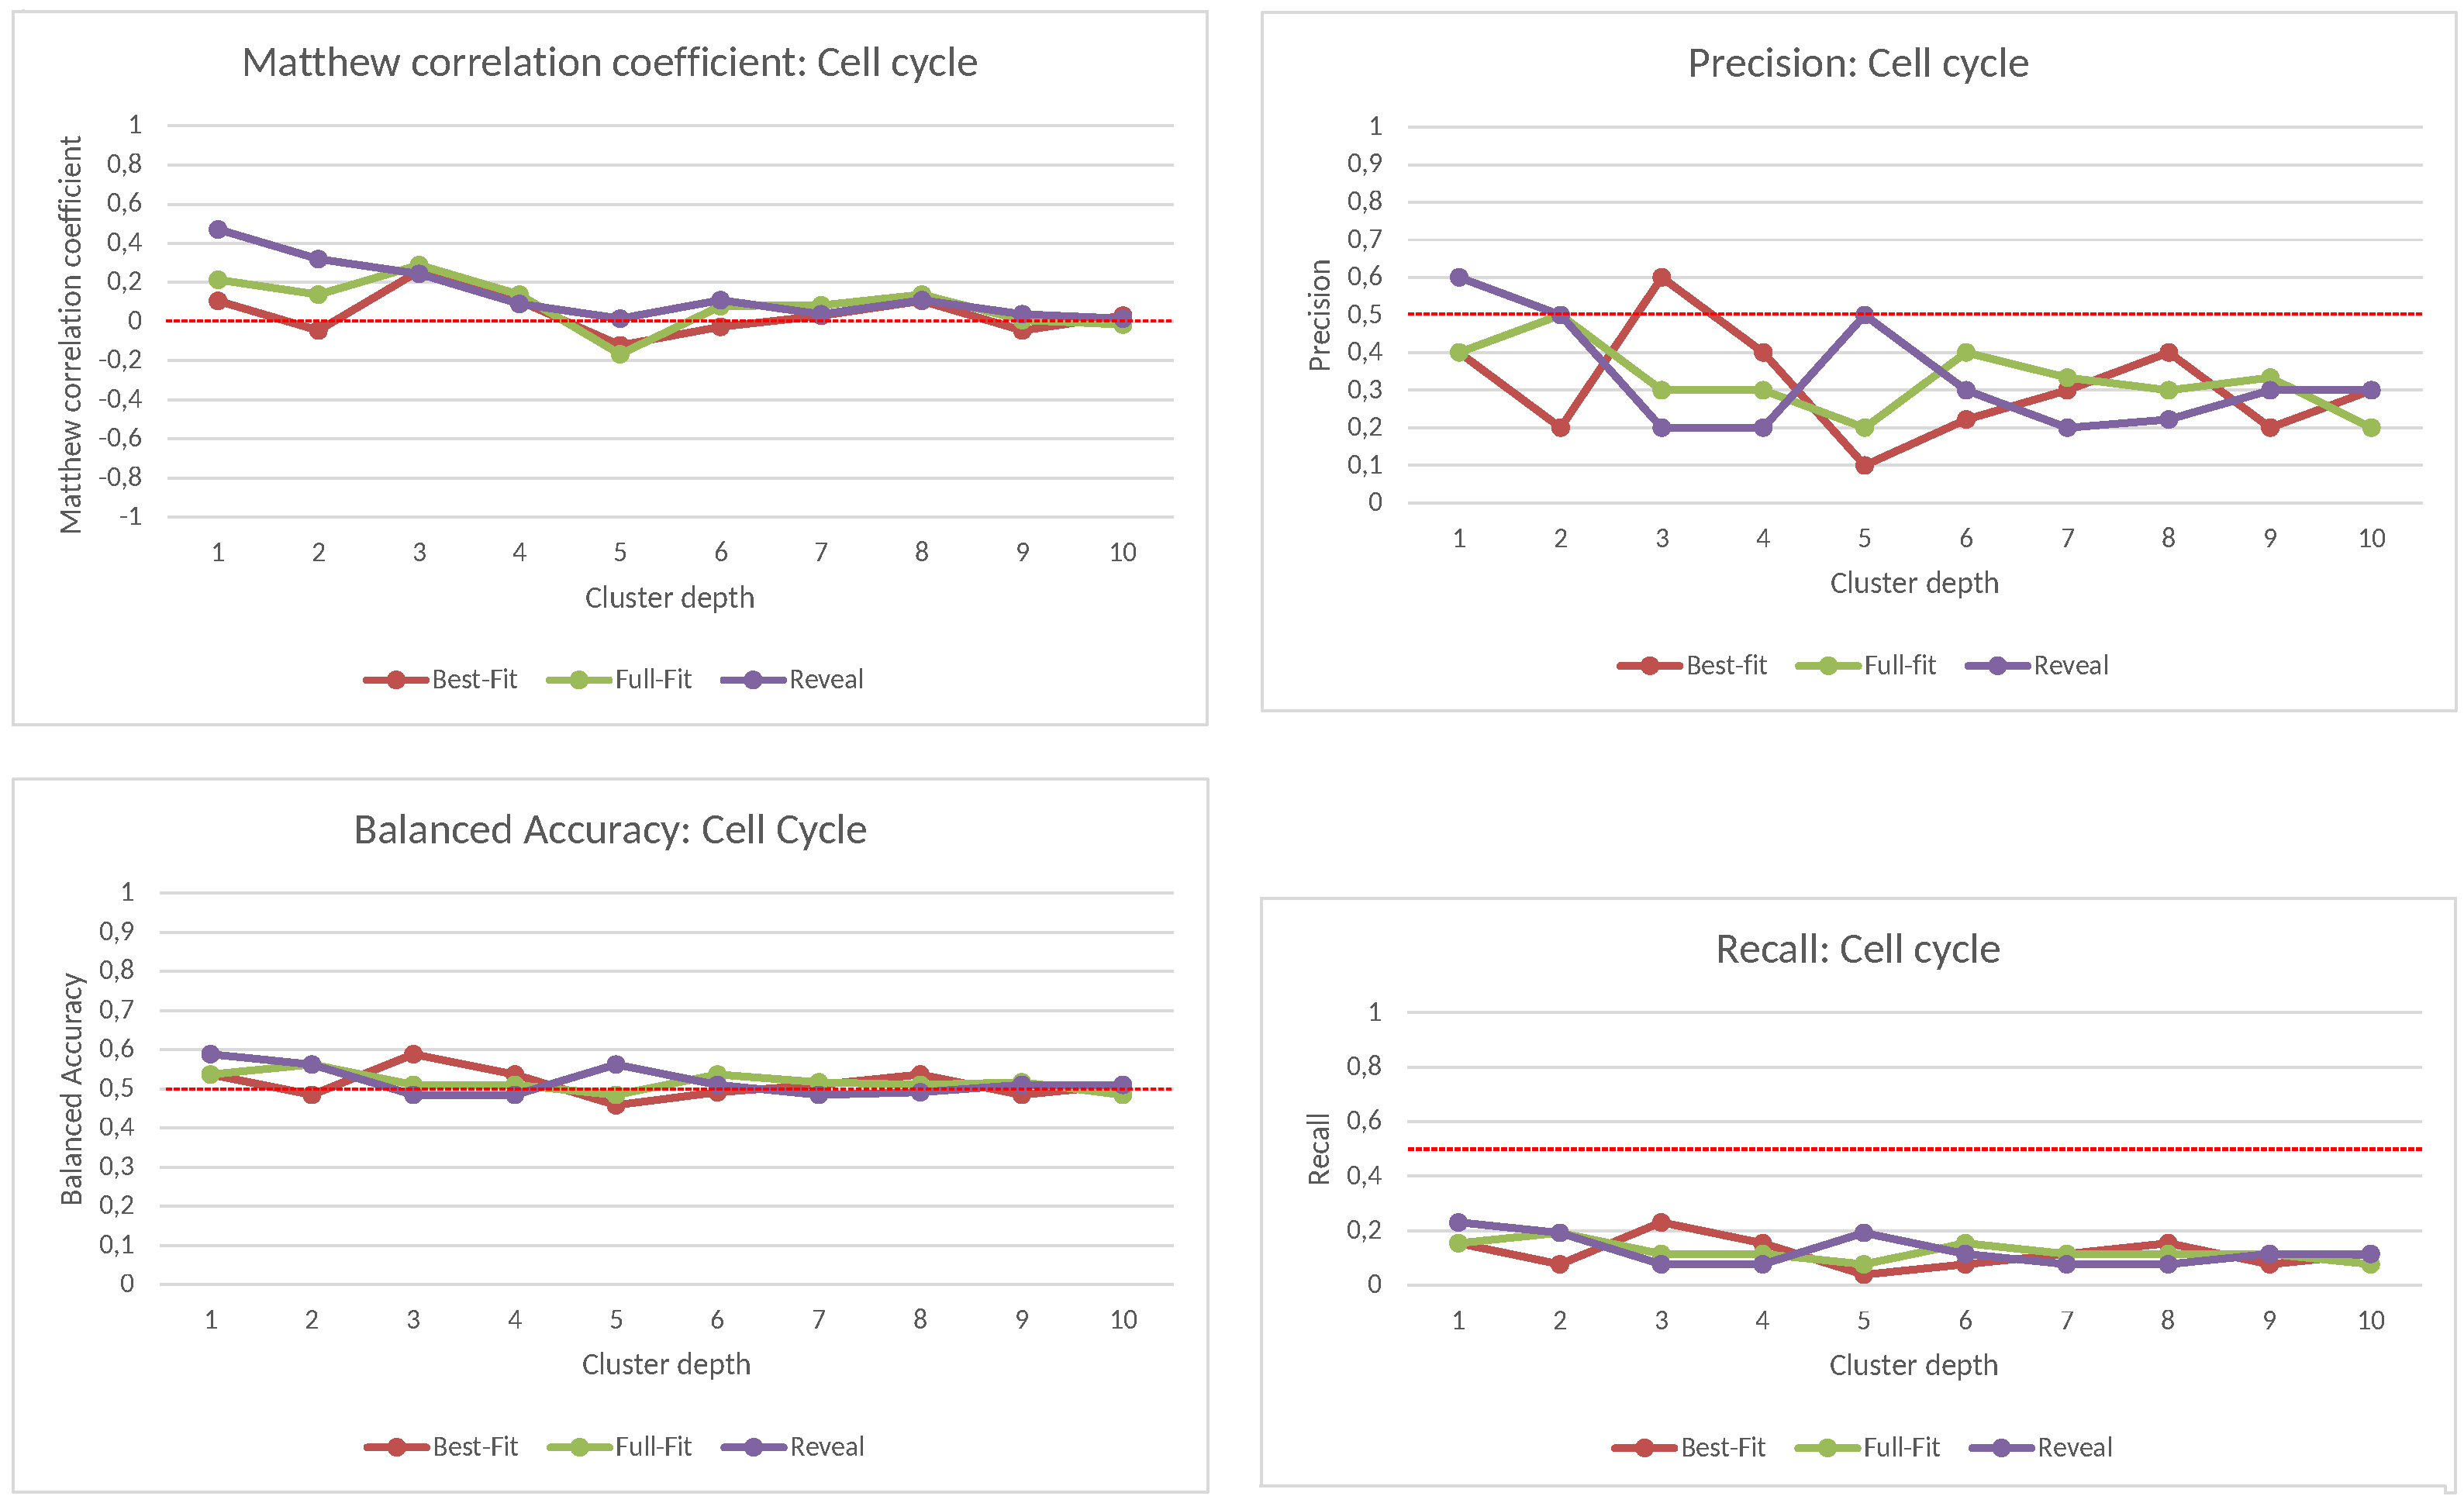
\includegraphics[width=1.0\textwidth]{./Bilder/Scoring/insilico/3_cellcycle_clusterdepth/insilico3.pdf}
\caption[Clusterdepth BCC]{For a clustering depth of $1$ to $10$ the three algorithms are performed resulting in a balanced accuracy that ranges around a value of $0,5$. Changing the clustering depth causes no significant change in the network performance.}
\label{fig:7}
\end{figure}

\section{Pipeline of the Dream8 Challenge data set}
\begin{figure}[H]
\centering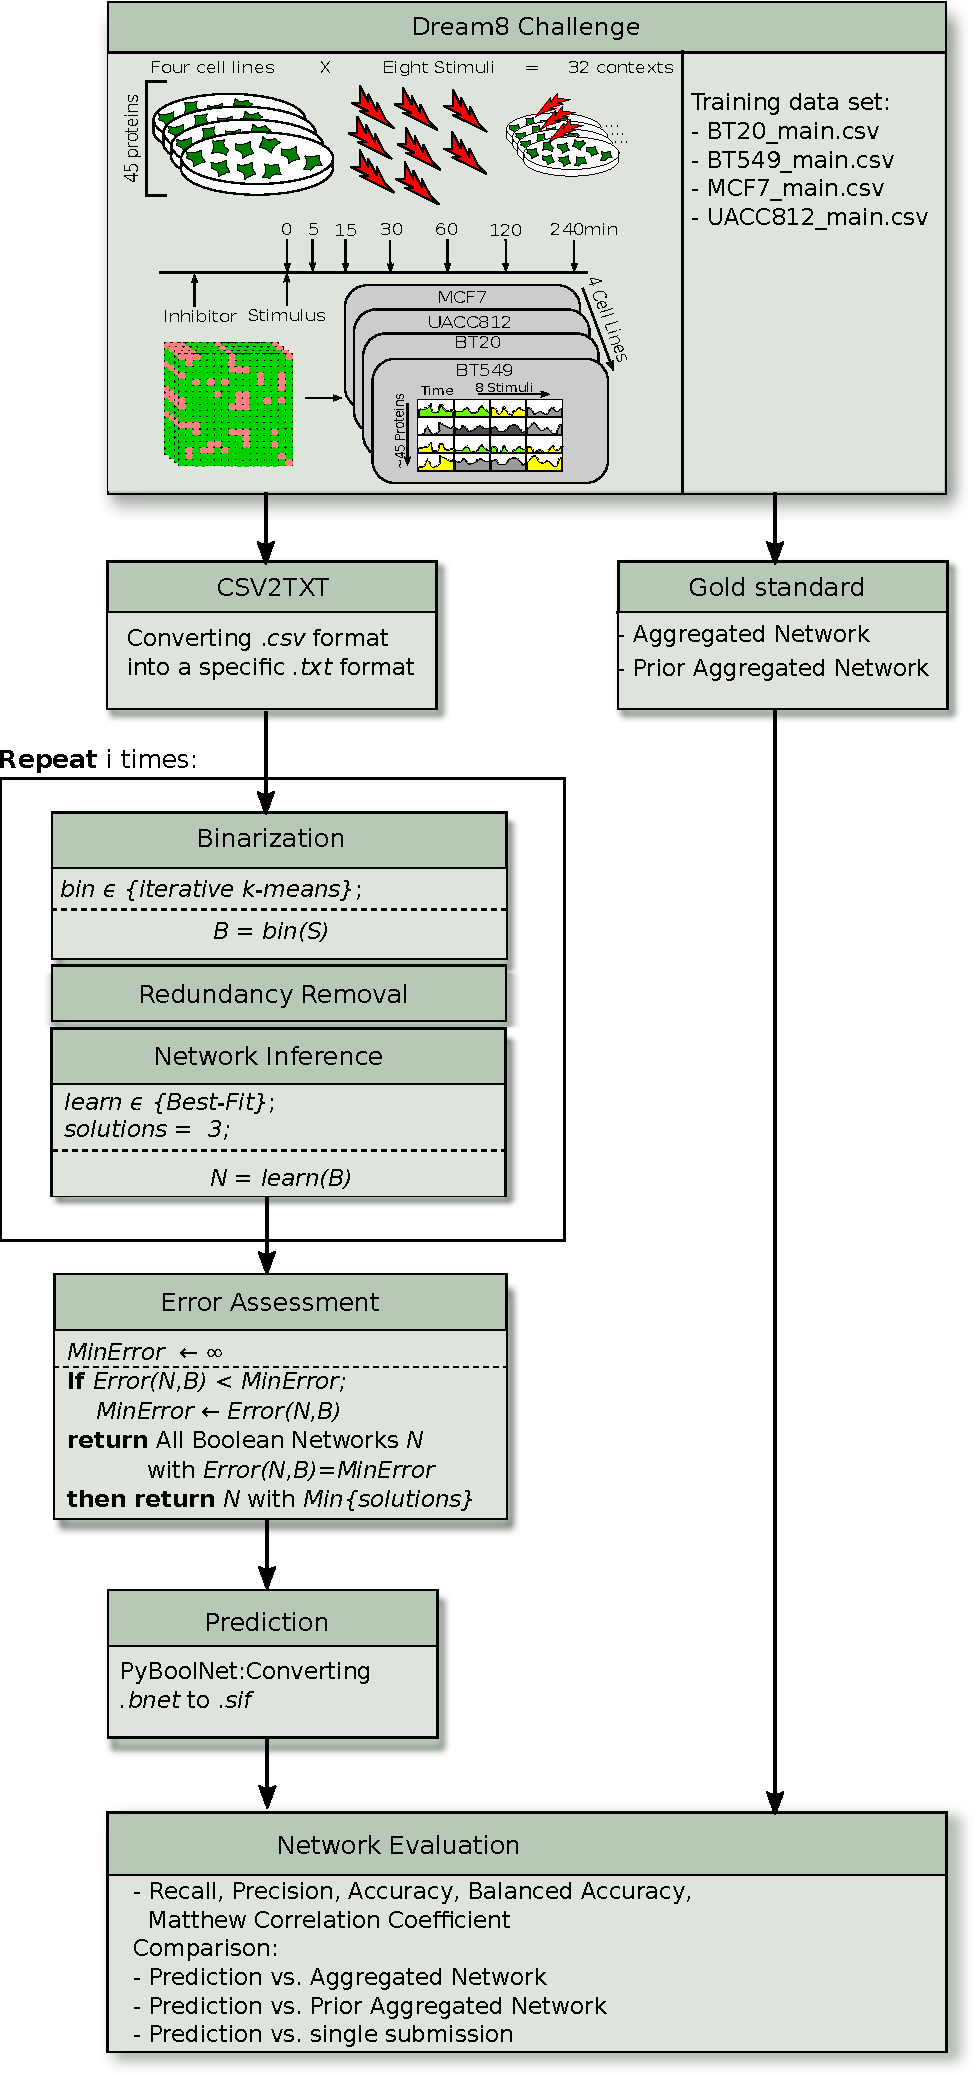
\includegraphics[width=0.6\textwidth]{./Bilder/pipeline_dream8.pdf}
\caption[pipelineDream8]{\textbf{Pipeline Dream8 Challenge. }}
\label{fig:9}
\end{figure}

%Raw structure
%-Pipeline fast identisch in silico pipeline mit einzigen Unterschied: input datensatz, km3+bestfit und gold standard selection.

%Learn-method: BESTFIT wird benutzt, weil: aus in silico weiß man, dass es mit fullfit gleich auf ist und durch das TS2B Paper, dass es die beste performance hat. 
% Prediction is converted to .bnet format for .sif format
%Goldstandard: welchen goldstandard hat die challenge verwendet und welchen gold standard benutze ich?
% Scoring gegen Prior aggregated network, aggregated network und letzten aus dem leaderboard(soll zeigen, dass Daten unbalanced sind), Erklären, warum ich mein eigenes Scoring mache und nicht dreamtools verwenden kann.
%Threshold: Wenn ich mehrere solutions habe, dann edge score berechenen über die Häufigeit von auftretenden Kanten, dann threshold verschieben, sodass von wenig bis viele tp sich ergeben = AUROC / = AUPR (Wegen runtime nicht gemacht,aber ich dann es ja für nur 3 runs zeigen?)


%Create 32 data set from training data -> txt. file
The 'main' training data set of the Dream8 Challenge is converted into a text file format (Figure 2.8, Figure 3.1) by splitting each data set of a cell line into eight text files depending on the stimulus. Each of the resulting 32 text files contain about $\sim $85 sample points and about $\sim $45 antibody names (Figure 3.8).\\

\subsection*{Network inference}
%Quelle: TS2B Paper mit KM3 Empfehlung
%The python implementation of the inference algorithms is validated, such that a network up to 50 nodes can be inferred and the 
%Network inference: KM3+Best-Fit
The higher the \textit{in-degree} of the nodes and the amount of nodes in a network the higher is the complexity in a system and the higher is the computational cost of an inference algorithm. Due to computational limitations and a technical settings of 8 RAM and a Core i5 processor the application of Reveal to the Dream8 Challenge data set is an infeasible task. 
Furthermore, results of the \textit{in silico} data set show that the choice of cluster depth abundance of sample points have no significant influence on the performance. An increasing \textit{in-degree} shows an decreasing performance for all three algorithms, such that no algorithm can be excluded by this investigation. Thus, results of (Paper Quelle) regarding error assessment are taken into account, such that a recommanded combination of Best-Fit with the iterative k-means algorithm with a $d=3$ is applied to the Dream8 Challenge data set. This combination yielded the best performance , especially in complex systems.\\
Predicted Boolean networks (\textit{bnet}) are converted into an Interaction graph (\textit{sif}) (Figure 4.2) and scored against a gold standard (Aggregated Network, Prior Aggregated Network). 
%Paper:TS2B Paper 
%Mit Fullfit auch das Scoring machen.

\subsection*{Gold standard selection}
%Goldstandard der challenge 
%Wie wird in der challenge gescored und (testdatensatz und AUROC AUPR, und wie score ich: Aggregated Network, Prior Aggregated Network, kein kantengewicht, kein threshold, daher Recall, Precision,....)
Network inference methods are often assessed using data simulated from known causal network structure, so called "gold standard network". It is useful to include prior knowledge, but this can come along with limitations, because it is difficult to truly mimic specific bilogical systems of interest. Learning novel connections in a network is restricted by comparing inferred networks to literature. For this purpose no gold-standard is provided in this Dream Challenge.  For testing the algorithms an \textit{in silico} data set is provided and prior knowledge independent network can be created with the training data set of the experimental data. The \textit{in silico} data set is generated from a nonlinear ordinary differential equations (ODE) model of the ERBB signaling pathway (ERBB:family of proteins containing four receptor tyrosine kinases, structually related to the epidermal grwoth factor receptor (EGFR)). Nevertheless pre-existing biological knowledge was included by several participants and seemed to be broadly benefical. The predicted networks from the training data were assessed by the test data.
After finishing the challenge an Aggregated Network for all 32 contexts was submitted. These aggregated networks are a compendium of 66 submissions of the participants of this challenge with the best performance reduced by correlated submissions.
%Paper: Dream8 Challenge über aggregated networks
Furthermore an Aggregated Prior Network is provided, a combination of 10 prior knowledge networks that teams used as part of their submission (Table 3.2). Hence, the aggregated network and the aggregated prior knowledge network are used in this thesis as a gold standard to test the performance of Best-Fit. Predictions of all 74 participants of the Dream8 challenge leaderboard are scored against the two aggregated networks,such that a new ranking including the new prediction by Best-Fit is determined.

\begin{table}[H]
%\resizebox{\textwidth}{!}{
%{\tabcolsep=6pt%
\begin{center}
%\captionsetup{width=0.87\linewidth}
%\small
\begin{tabular}{l|l|l}
\toprule 
Network & $\# $ Edges & $\# $ Networks\\
 \hline\hline
Prediction (Best-Fit) & $\sim 140$ & 1\\
\rowcolor{black!10} Aggregated Network & $\sim 2200 $ & 66\\
Aggregated Prior Network & $\sim 1400$ & 10\\
\bottomrule
\end{tabular}
\captionof{table}{Network structure}
\end{center}
%}
\end{table} 



\subsection*{Evaluation}
Due to different strategies of evaluating predictions, e.g. choice of the scoring metric and implementation approach, it is hard to compare the resulting performance between the participants. For this reason the Dream8 Challenge provides a standard scoring tool 'DREAMTools' Python package.
%Quelle:  \citep{Cokelaer T, Bansal M, Bare C et al. DREAMTools: a Python package for scoring collaborative challenges [version 2; referees: 1 approved, 2 approved with reservations]. F1000Research 2016, 4:1030 (doi: 10.12688/f1000research.7118.2)}
This tool needs as input a \textit{sif} and an \textit{eda} file, where eda (electronic design automation) contains the confidence scores of edges in an Interaction Graph. By these information dreamtools returns AUROC (area under the receiver operating characteristic curve)  and AUPR (area under the precision recall curve). AUPR is used for the case when there is an imbalance in the classes of the confusion matrix. Here a threshold $\tau$ is shifted, such that the true positiv value increases and a curve for both metrics are producible.
%Verweis auf Anhang: Erklärung/Definition von AUPR und AUROC
An idea is to run the pipeline several times, ideally about 100 times to get a sufficient set of confiodence score for the prediction. Then over the resulting set of predictions occurences of edges are count, such that a pobability of an edge occurence is obtained. As mentioned in 'Network inference' the computational power is limited. One execution of the pipeline needs about 5 hours. Of course it was taken into account to use a cluster (e.g. Allegro), due to a lack of globally implemented bioconda for installing Pycluster, this approach failed.
Therefore, just the performance of the algorithms concering inferring the interaction graph is performed, such that the scoring tool of the DreamChallenge can not be used. For this reason an own scoring script is implemented by comparing the interaction graph of the prediction against a gold standard returning the precision, recall, structural accuracy, balanced accuracy and Matthew corrlation coefficient. 

\newpage
\section{Results of the Dream8 Challenge data}
\subsection*{Prediction versus Aggregated Network and Aggregated Prior Network}
Scoring the prediction against the last participant of the leaderboard in the Dream8 Challenge (rank: 74.) ranges in the accuracy inbetween a value of 60\% to 80 \% (Figure 4.8). Scoring the prediction against the aggregated network yields are accuracy of 10\% to 18\%. This is du to the fact, that the cases of true negatives and true positives have a high imbalance. The application of the balanced accuracy shows that the previous observation has no significance of the performance.  
% High amount of FalseNegatives: Bad accuracy for prediction against aggregated network
% High amount of TrueNegatives: Good accuracy for prediction against aggregated network
%= Yield: Balanced accuracy is at random.
%Vllt. noch prediction vs. prior knowledge network mit einfügen
\begin{figure}[H]
\centering
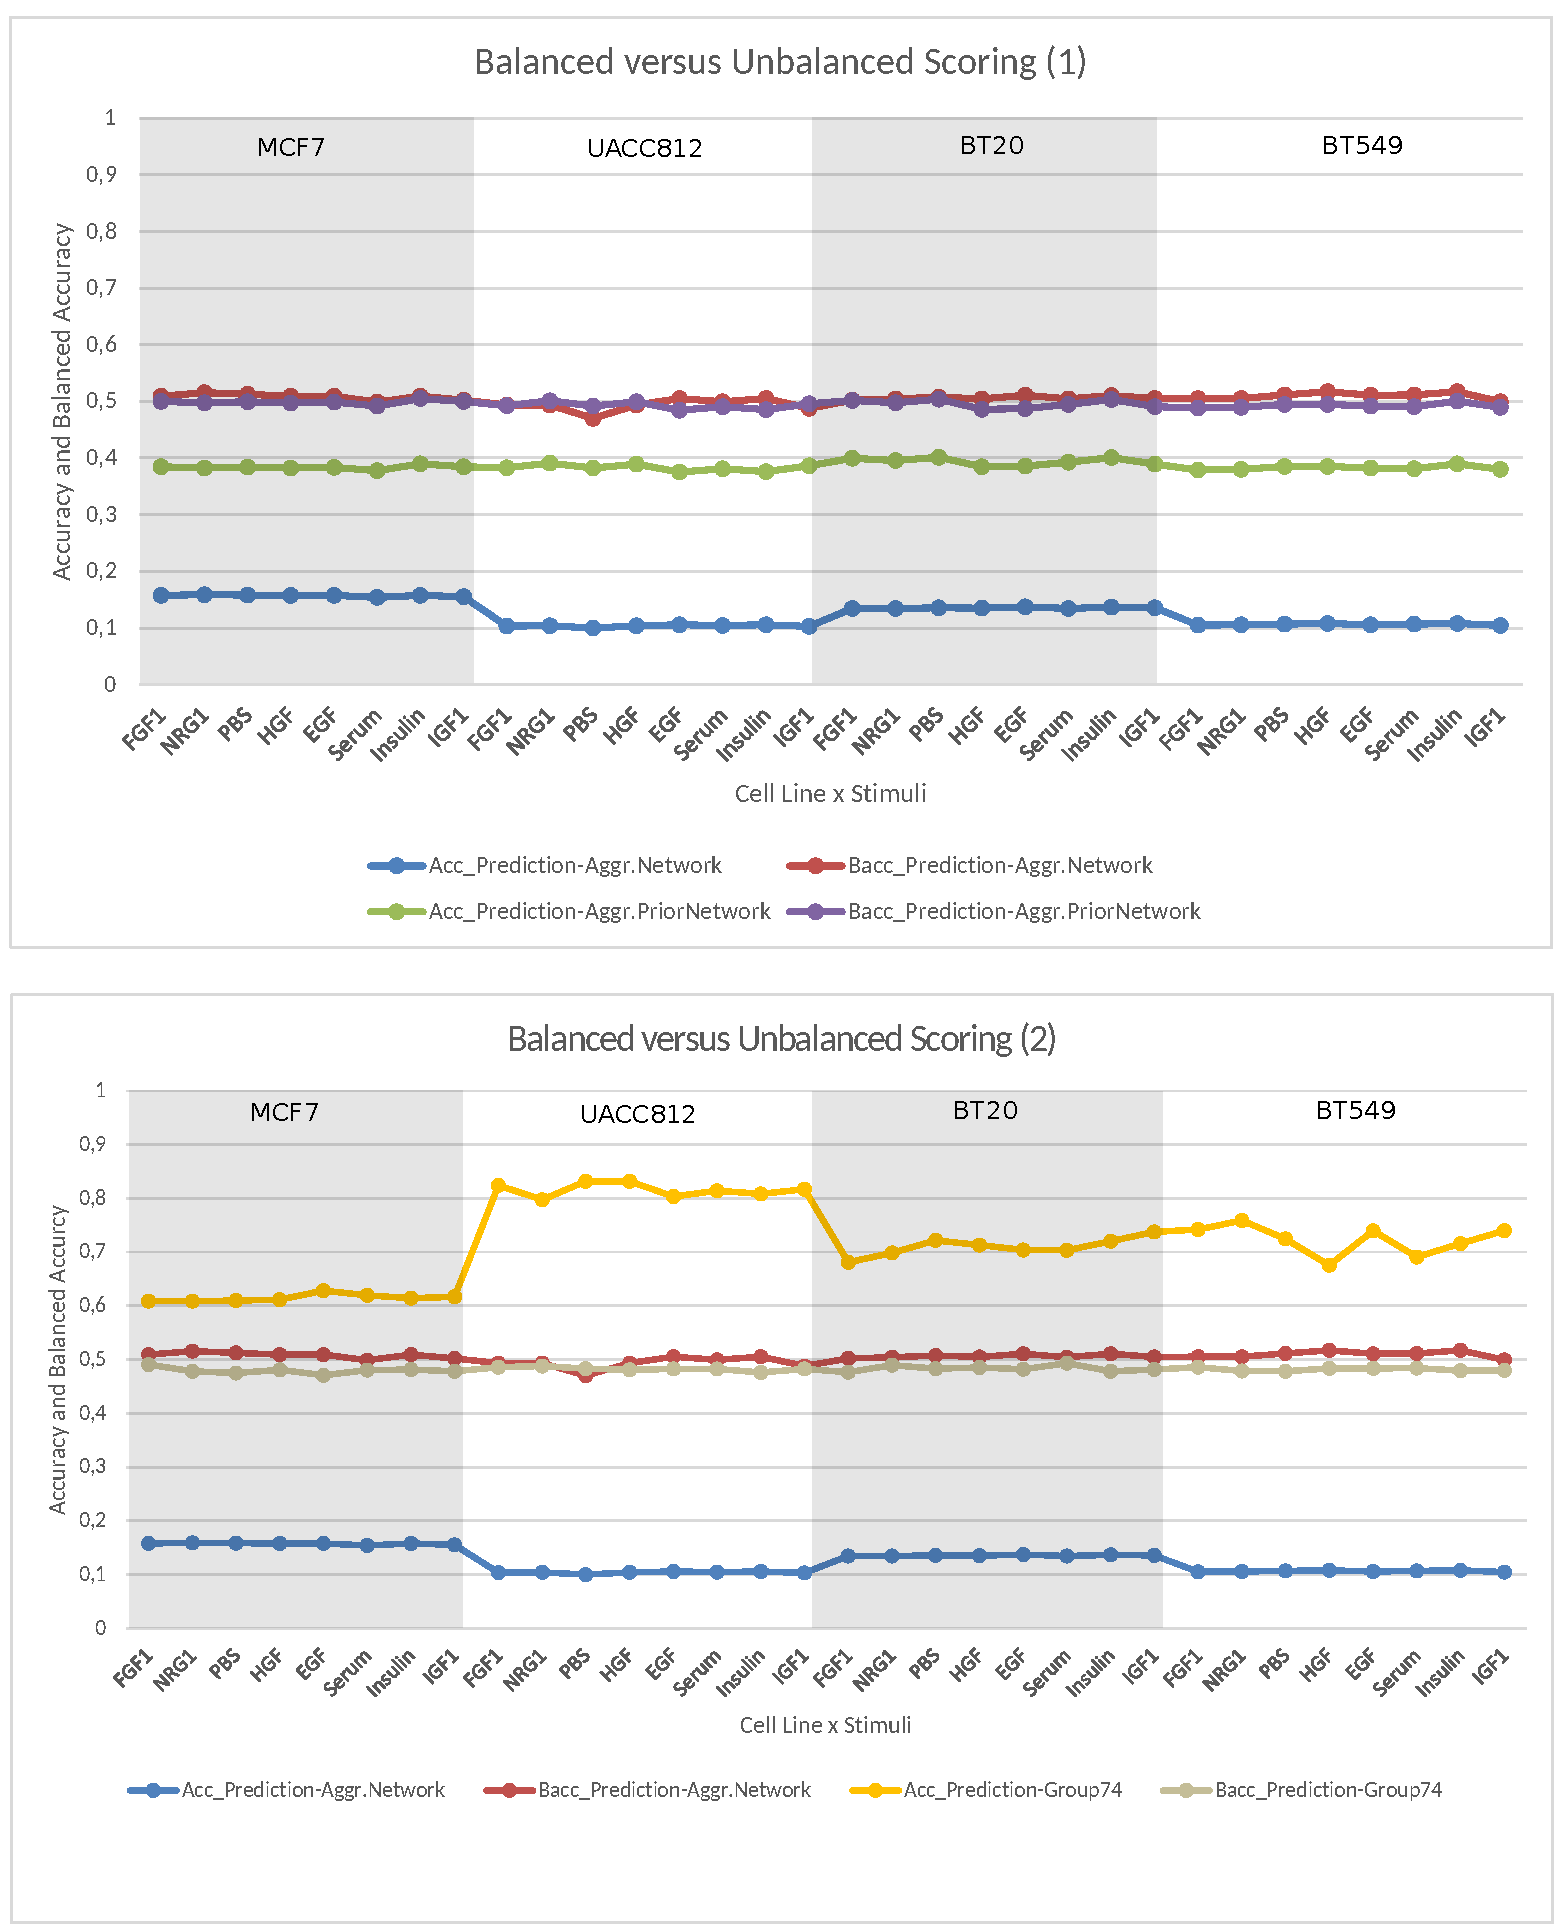
\includegraphics[width=1.0\textwidth]{./Bilder/Scoring/dreamchallenge/1_Balanced_vs_Unbalanced/balanced.pdf}
\caption[Blanced vs. Unbalanced]{Balanced versus Unbalanced. Accuracy and Balanced Accuracy for (1) Prediction scored against Aggregated Network and Aggregated Prior Network; (2) Prediction scored against Aggregated Network  and submission of the 74. participant of the Dream8 Challenge.}
\label{fig:10}
\end{figure}

\begin{figure}[H]
\centering
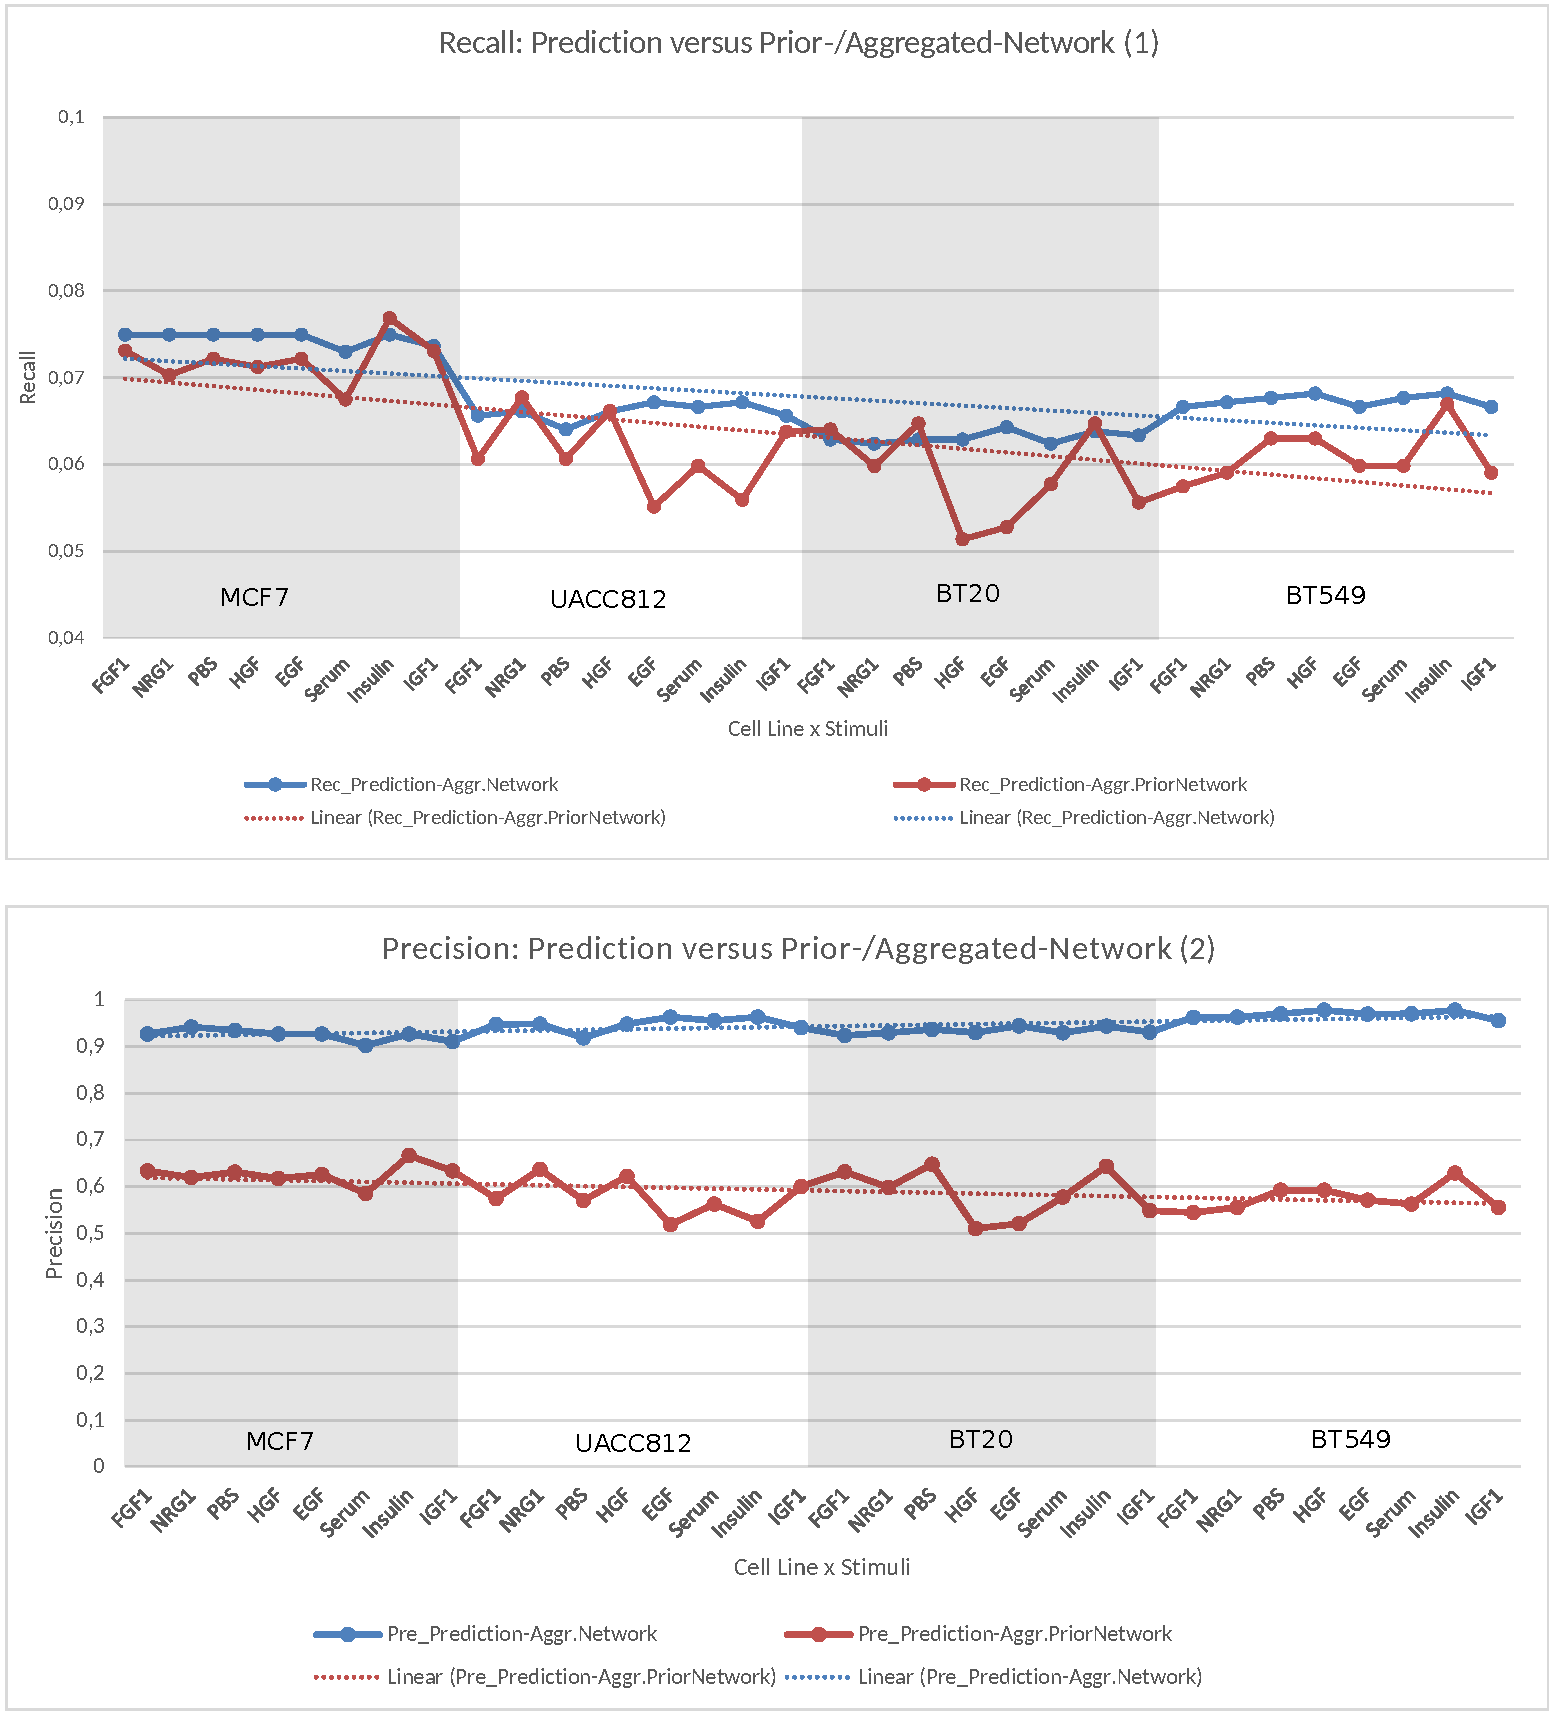
\includegraphics[width=1.0\textwidth]{./Bilder/Scoring/dreamchallenge/1_Balanced_vs_Unbalanced/balanced_rec_prec.pdf}
\caption[Recall and Precision: Prediction versus Aggregated/Prior Network]{Recall and Precision: (1) Prediction versus Aggregated Network and (2) Prediction versus Aggregated Prior Network}
\label{fig:10}
\end{figure}

\subsection*{New Ranking: Aggregated Network and Aggregated Prior Network}
%New ranking
%Noch scoring für: MCC für prediction + submissions gegen aggregated prior knowledge network

\begin{figure}[H]
\centering
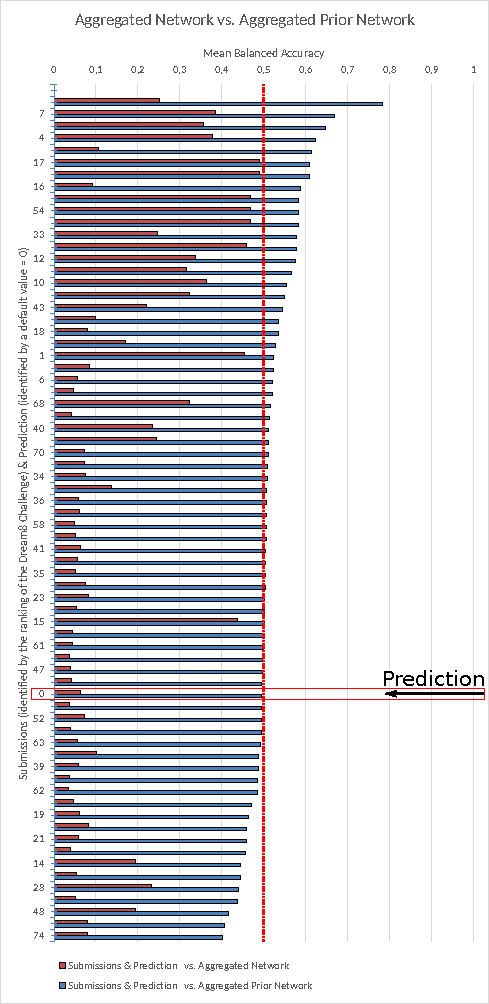
\includegraphics[width=0.62\textwidth]{./Bilder/Scoring/dreamchallenge/Meanbacc_vertical_comparison.pdf}
\caption[New Ranking (Balanced Accuracy): Aggr. Network and Aggr.Prior Network]{New Ranking: Aggregated Network and Aggregated Prior Network}
\label{fig:}
\end{figure}


%Hier noch precision,recall, acc, bacc einfügen?
%Angeben welchen Platz diePrediction nach dem neuen Ranking hätte
%scoring der prediction gegen das AggregatedPrior Knowlede network




